\newpage
\section{Funzionamento del prodotto}

PotNet è dal punto di vista tecnologico un prodotto relativamente semplice da realizzare e che non richiede particolari tecnologie hardware o software. 

\subsection{Hardware}

Il prototipo fisico realizzato, ha previsto l'utilizzo dei seguenti componenti:

\begin{itemize}
	\item \textbf{Raspberry PI 2 Model B[30€]:} microcontrollore per la lettura dei sensori, mantenimento dello stato e comunicazione con il server centrale;
	\item \textbf{DHT11[1.5€]:} sensore di temperatura e umidità ambientale;
	\item \textbf{Fotoresistore[0.5€]:} sensore di luminosità ambientale;
	\item \textbf{Batteria da 5000mAh[5€]:} per poter utilizzare il dispositivo senza doverlo tenere sempre collegato alla corrente;
\end{itemize}

Per il prodotto destinato alla vendita non utilizzeremo più una Raspberry PI, la quale ha un costo, potenza computazionale e un consumo decisamente più alti di quelli a noi necessari. Si renderebbe quindi necessaria la progettazione e realizzazione di una board ad hoc con i sensori già integrati in essa. In questo modo si andrebbero a ridurre notevolmente i costi di produzione, l'ingombro e il consumo energetico. A sua volta, anche la capacità della batteria potrebbe essere ridotta, contenendo ancor di più le dimensioni, il peso e il costo del prodotto. PotNet risulterebbe grande meno della metà del prototipo (indicativamente 6 x 3 x 1.5 cm), un peso inferiore ai 200g e un'autonomia stimata di circa 14-20 giorni.

\subsection{Software}

A livello software, il dispositivo rileva i dati dei sensori ad intervalli prestabiliti e ne mantiene lo storico in memoria. Inoltre, si connette al server centrale il quale si occupa di far da tramite tra i dispositivi e le varie interfacce tramite cui l'utente può tenersi informato sullo stato della pianta (Bot Telegram, Alexa, Web UI).\newline\newline Il software del server centrale risiederà su un servizio come ad esempio Amazon AWS. Questo ci permetterà di avere un servizio affidabile, scalabile e di risparmiare soprattutto nella fase iniziale del progetto, in cui sarebbe insostenibile economicamente creare una nostra infrastruttura, ma senza rinunciare ad avere un servizio di qualità.

Il software necessario al funzionamento di PotNetBot, della skill di Alexa e della Web UI comunica con il server centrale per acquisire i dati richiesti dall'utente e permettendo un sistema di notifiche rapido nel caso di valori fuori soglia. 

\newpage
\subsection{Prima architettura logica}

La figura \ref{fig:logical_arch} mostra una prima architettura logica di riferimento del sistema software, composto da più parti:
\begin{itemize}
	\item \textbf{PotNetCore}: insieme di servizi in esecuzione sul dispositivo PotNet;\footnote{\url{https://github.com/LM-96/Greengers/tree/main/PotNetCore}}
	
	\item \textbf{PotNetCentral}: server centrale (\textit{middleware});\footnote{\url{https://github.com/LM-96/Greengers/tree/main/PotNetCentral}}
	\item \textbf{PotNetUI}: interfaccia utente (generica);
	
	\item \textbf{PotNetAlexaSkill}: servizio per le funzionalità Alexa;
	
	\item \textbf{PotNetBot}: servizio per le funzionalità del bot Telegram;\footnote{\url{https://github.com/m-dilorenzi/prova-vaso-smart}}
	
	\item \textbf{PotNetBotClient}: interfaccia utente per il bot Telegram.
\end{itemize}

\begin{figure}[h]
	\centering
	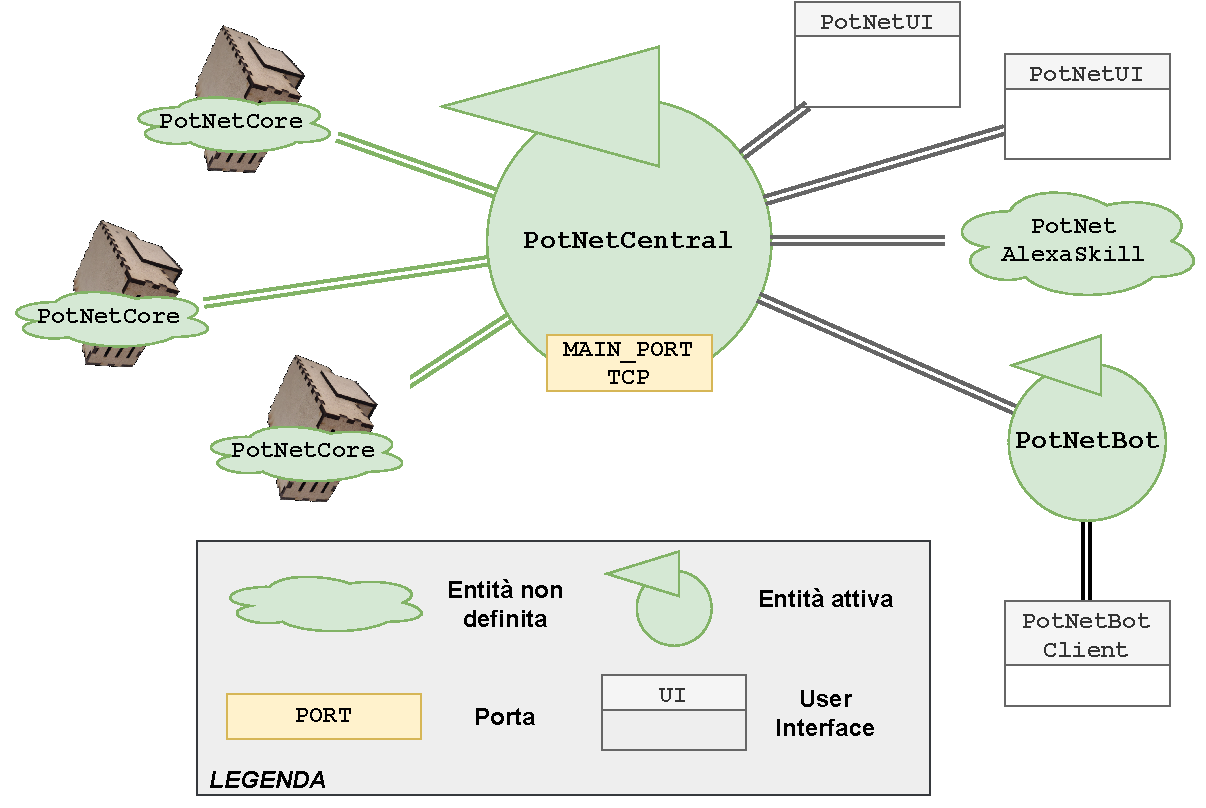
\includegraphics[scale=0.8]{images/logical_arch.pdf}
	\caption{Prima architettura logica del sistema software}
	\label{fig:logical_arch}
\end{figure}

Tale architettura logica verrà impiegata in fase di prototipazione, insieme ai sorgenti principali (in Kotin e NodeJS), senza precludere però la possibilità di successive modifiche in una fase più avanzata.

Inoltre, per le parti di codice in Java/Kotlin, è stata pensata la libreria \textit{PotConnectors}\footnote{\url{https://github.com/LM-96/Greengers/tree/main/PotConnectors}} per la gestione delle connessioni e piccole funzioni di utilità: tale libreria è utilizzata nelle prime build di \textit{PotNetCore} e \textit{PotNetCentral}.

\newpage
\subsubsection{Modularità}

Tutte le parti software sono state pensate e realizzate per essere modulari. In questo modo, il tempo per aggiungere, modificare o migliorare le funzionalità sarà il più breve possibile e permetterà al team di sviluppo di intervenire tempestivamente per risolvere eventuali problemi o introdurre funzionalità richieste dai clienti.
\newline Anche lo sviluppo di nuovi modelli di PotNet ne beneficerà, in quanto tutto il software già realizzato per la prima versione potrà essere riutilizzato ed esteso per comunicare con i nuovi sensori. Questo si tradurrà in un minor dispendio di tempo (e quindi economico) e una maggior qualità del software.
\newline\newline Anche i servizi offerti potranno essere ampliati, infatti il software è stato scritto in modo da poter essere facilmente e velocemente espandibile ed integrabile con altri servizi in futuro. Alcuni esempi potrebbero essere il supporto di diversi assistenti vocali oltre ad Alexa, lo sviluppo di un'app apposita per Android e iOS e l'integrazione con protocolli IoT standard.